\subsection{Solving the risk sensitive POMDP}

\normalsize
Marecki \cite{marecki} showed that RSPOMDPs can be solved for arbitrary utility functions using \textbf{reverse value iteration} in Belief Wealth Space.
For this the original state space must be augmented two times:

\begin{figure}
\begin {center}
\begin {tikzpicture}[-latex ,auto ,node distance =4cm and 2cm ,on grid,
semithick , state/.style ={ circle ,fill=black!20, minimum width =3 cm}]
\node[state] (A) [align=center] {Observation\\Time\\Space};
\node[state] (B) [right of=A,align=center] {Belief\\Time\\Space};
\node[state] (C) [right of=B,align=center] {Belief\\Wealth\\Space};


\path (A) edge [line width=2mm, align=center] node[left] {} (B);
\path (B) edge [line width=2mm,align=center] node[below =0.25 cm] {} (C);
\end{tikzpicture}
\end{center}
\end{figure}

\hspace{2cm}

\subsection{Value functions in belief wealth space}


\normalsize

\begin{figure}
    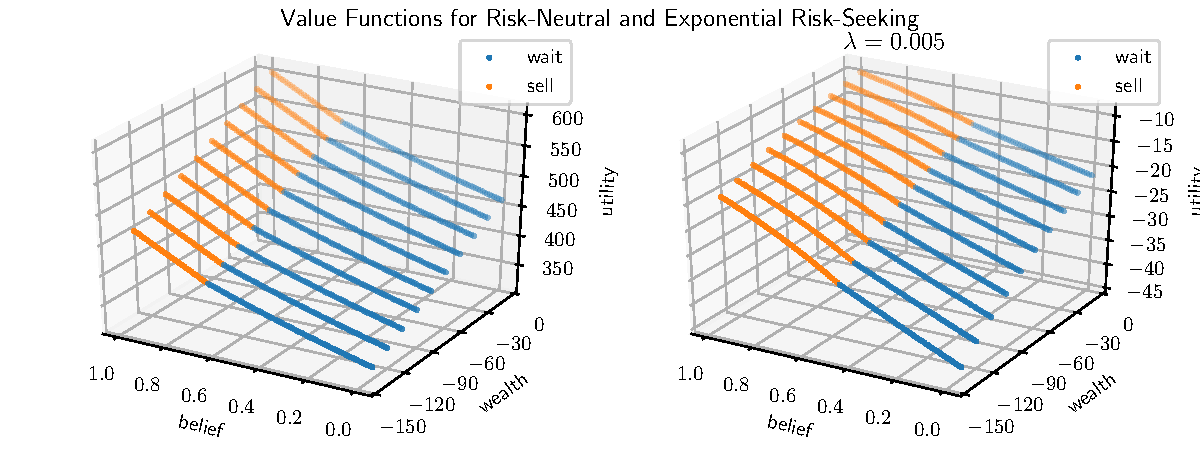
\includegraphics[width=0.98\linewidth]{img/exp_policy.pdf}\\
    \vspace{1cm}
    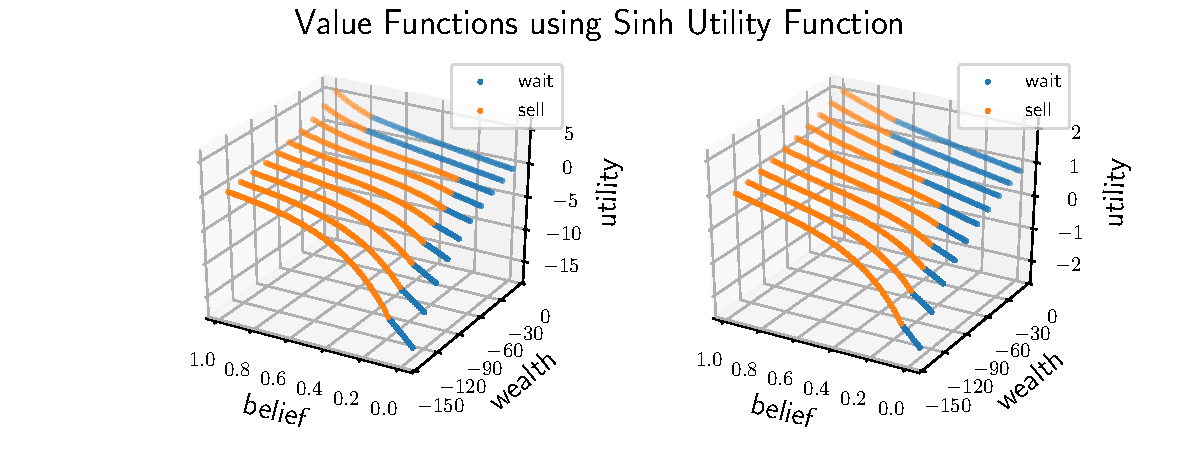
\includegraphics[width=0.98\linewidth]{img/sinh_policy.pdf}\\
    \vspace{1cm}
    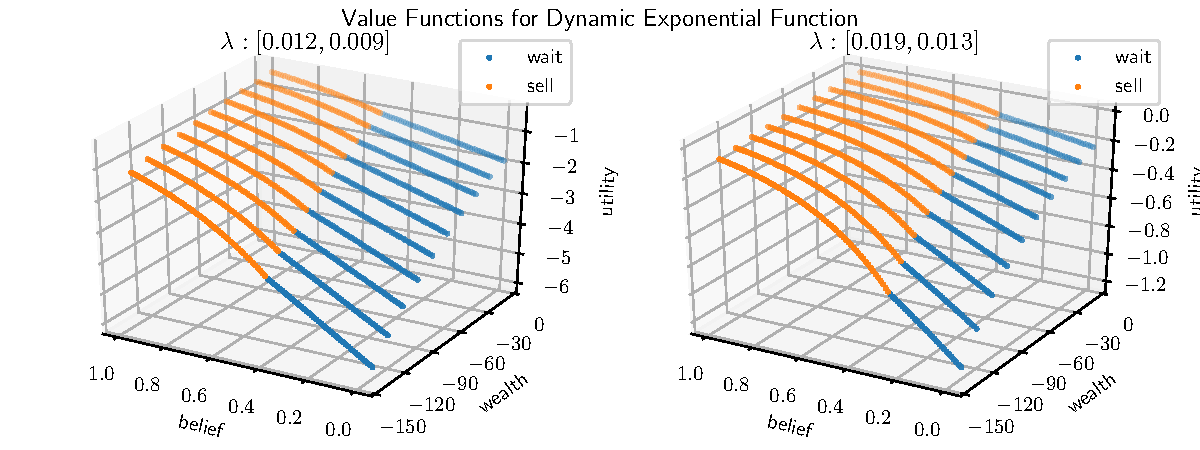
\includegraphics[width=0.98\linewidth]{img/dyn_policy.pdf}
    \caption{Value functions exhibiting different risk-behaviors; from top left: risk neutral agent (utility function is the identity function), risk-seeking agent with exponential utility function, two fixed time agents with different time thresholds, two agents with dynamic exponential utility function.}
\end{figure}

\subsection{From human behavior to utility functions}


\normalsize
\textbf{The original problem:}
\begin{itemize}
\item[①] Choose utility function with risk parameter.
\item[②] Perform value iteration.
\item[③] Derive policy.
\end{itemize}

\textbf{The inverse problem:}
\begin{itemize}
\item[①] Observe behavior.
\item[②] Estimate policy.
\item[③] Derive utility function and risk parameters.
\end{itemize}

The original problem is easy to solve, unfortunately for the inverse problem no solution is known. 

$\rightarrow$ Perform grid-search and choose optimal utility function.

\begin{figure}
    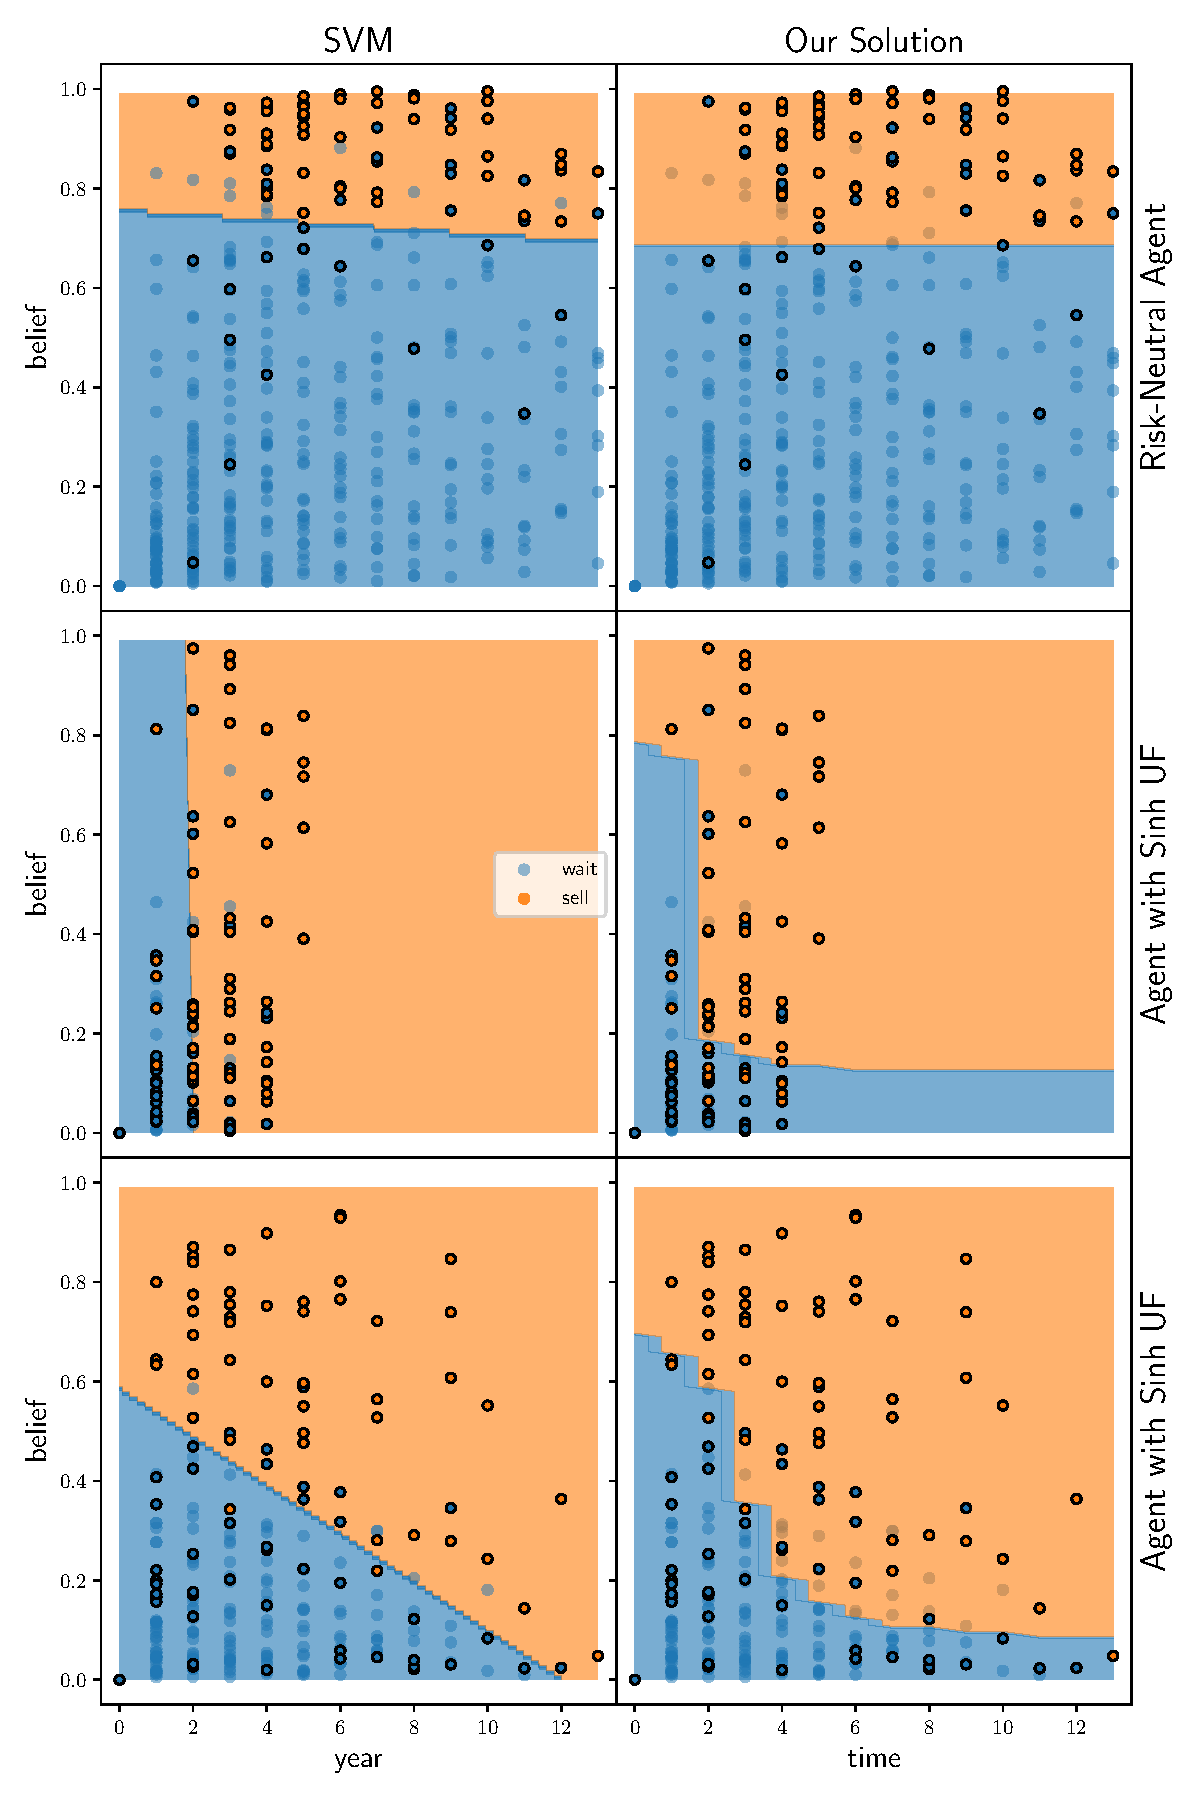
\includegraphics[width=0.8\linewidth]{img/fit}
    \caption{Examples from three human behaviors distinctly observed and replicated with RL agents. Behaviours by row: 1) Constant belief threshold, modelled by exponential utility, 2) Fixed time threshold, modelled by sinh utility, 3) Mixed strategy, modelled by dynamic exponential utility. Left column shows empirical optimal split of data using cross validation and linear kernel support vector machines, right column shows optimal policy found via gridsearch.}
    \label{fig:svm_vs_value}
\end{figure}

% TODO 6 boxes with only expensive expert and 3 behavior clusters.

\begin{figure}
% 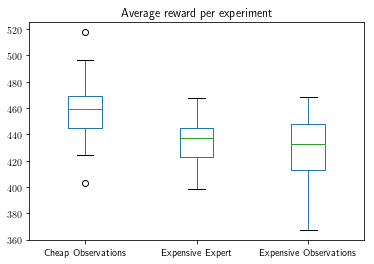
\includegraphics[width=0.4\linewidth]{img/avg_reward.png}
% 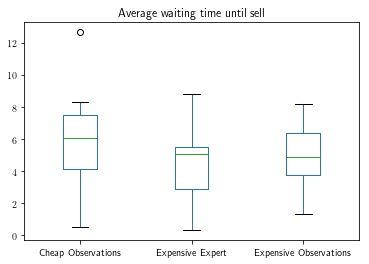
\includegraphics[width=0.4\linewidth]{img/avg_waiting.png}
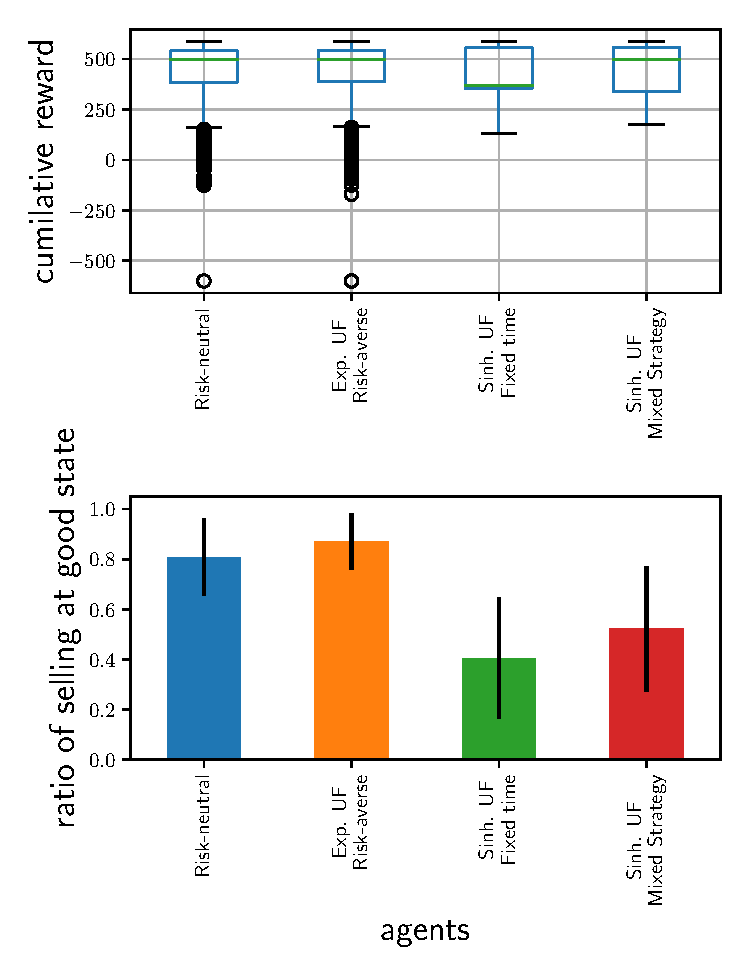
\includegraphics[width=0.8\linewidth]{img/performance.pdf}
\caption{Average reward and ratio of selling in the good state.}
\end{figure}
